% !TEX root = ../notes_unsupervisedlearning.tex
% Chapter 8: Zero-Shot, Few-Shot, and Transfer Learning
%%%%%%%%%%%%%%%%%%%%%%%%%%%%%%%%%%%%%%%%%%%%%%%%%%%%%%%%%%%%%%%%%%%%%%

\chapter{Transfer Learning}\index{Zero-Shot}\index{CLIP}\index{Transfer Learning}\index{foundation model}\index{backbone}
\newthought{The Flywheel of Generalized Embeddings.}

%═══════════════════════════════════════════════════════════════════════
% CHAPTER 08 SCOPE (agreed in scoping session 2026-04-26)
%═══════════════════════════════════════════════════════════════════════
% ARCHETYPE: ch06 introduce-then-upgrade arc.
% SPINE:     embeddings -> backbones -> foundation models -> capabilities -> composing.
%
% Block 2 sections, in order:
%
%   1. Embeddings, Backbones, Foundation Models
%      Origin story: hand-crafted features -> ImageNet supervised pretraining
%      (Razavian 2014, Yosinski 2014) -> web-scale pretraining -> foundation models.
%      Pretraining-dataset table (already drafted in iffalse-block, keep).
%      "Notice that": foundation models are backbones plus scale plus breadth
%      plus often cross-modal alignment, no new architecture.
%
%   2. The Transfer Continuum
%      One axis: frozen feature extraction -> linear probing -> partial fine-tuning
%      -> full fine-tuning -> PEFT -> prompting -> in-context learning.
%      Origin for PEFT (LoRA-centric): full FT infeasible at billion params.
%      Recipe box: data regime x domain gap -> strategy. (Hyperparameter-as-bridge.)
%      Failure-mode beat with heading: negative transfer + catastrophic forgetting.
%      Domain shift as closing sub-paragraph of failure beat: covariate /
%      label / concept shift in two sentences each, adversarial DA in one
%      sentence with margin pointer. NOT its own section.
%
%   3. Zero- and Few-Shot Learning
%      Origin (Lampert 2009): attribute-based zero-shot needed a hand-built
%      class-attribute table; this explains why zero-shot needs a bridge
%      between class semantics and image features, which is exactly what
%      CLIP supplies in section 4.
%      Few-shot recipes in the embedding space: linear probe with K shots,
%      prototypical / nearest-class-mean.
%      In-context learning named as the no-gradient few-shot mode, with a
%      marginnote pointer that ICL details belong to the LLM lecture series.
%      Prompt engineering and CoOp (table already drafted in iffalse-block).
%      LLM-PROMPTING THUMBNAIL [added 2026-04-27]: a tight historical
%      sketch of how the field went from naive prompting to aligned models:
%      raw next-token prediction (Brown 2020 GPT-3) -> chain-of-thought
%      prompting (Wei 2022) -> soft / prompt tuning (Lester 2021,
%      Li & Liang 2021) -> instruction tuning (Wei 2021 FLAN, Sanh 2021 T0)
%      -> RLHF (Christiano 2017, Ouyang 2022 InstructGPT) -> DPO and
%      successors (Rafailov 2023). Keep the thumbnail to 1-2 newthought
%      paragraphs; the full LLM story belongs to the LLM lecture series.
%      The point is to give students the names of the steps and a one-line
%      framing of each, not derivations.
%
%   4. CLIP and Cross-Modal Alignment
%      Contrastive image-text objective, diagonal-loss training figure,
%      one worked zero-shot classification trace.
%      TRIM: SigLIP / ALIGN / BLIP collapse into ONE marginnote.
%      Multimodal LLMs / VLMs in a separate marginnote pointing at the LLM series.
%
%   5. Composing Foundation Models
%      CENTERPIECE: Retrieval-augmented generation (RAG). An embedding
%      backbone (callback to §1) encodes documents and queries; similarity
%      search retrieves relevant context; a frozen generator consumes the
%      retrieved context to produce an answer. RAG is the canonical
%      composition pattern: knowledge added at inference instead of in
%      training, the alternative end of the transfer continuum (§2).
%      Other compositions to mention briefly: CLIP for retrieval + SAM
%      for segmentation + an LLM for reasoning, in a single pipeline none
%      of them was trained for.
%      Use-payoff that closes the algorithmic arc (the equivalent of ch06
%      latent interpolation).
%      Marginnote teaser to ch14 (vision-language-action models).
%
%   6. AI Engineering  [added 2026-04-27, RAG repositioned to §5 same day]
%      Theme: concepts that matter when we reuse and DEPLOY large models
%      we cannot really control through training. Sits at the bottom of
%      Block 2 as the operational counterpart to the algorithmic content
%      in §1-§5.
%      Tentative beats: shift from training to operating; tool use and
%      agents (give the model actions at inference; function calling,
%      agentic loops, multi-step orchestration); evaluation when you
%      didn't train (LLM-as-judge, behavioural / red-team tests, eval
%      harnesses, A/B in production); guardrails and safety (input/output
%      filters, refusal, jailbreak resistance, content moderation); cost /
%      latency / quality trade-offs (model selection, caching, speculative
%      decoding, distillation, quantisation); monitoring and drift
%      (callback to ch07); versioning, lineage, model cards, dataset cards.
%      RAG itself lives in §5 as the canonical composition pattern; §6
%      may reference RAG briefly when discussing engineering concerns
%      (chunking, vector stores, hybrid search) but does NOT own RAG.
%      Pedagogical move: widens Block 2 from "how to adapt a model" to
%      "how to operate one in production", which is where most students
%      will actually encounter foundation models.
%
% CENTER STAGE concepts every student leaves with:
%   backbone, foundation model, the transfer continuum, cross-modal alignment
%   for zero-shot, few-shot, composing foundation models, AI engineering as
%   the deployment-layer discipline above all of the above.
%
% MARGINNOTE-ONLY mentions (named, not derived):
%   PEFT siblings (adapters, BitFit, prompt tuning),
%   CLIP siblings (SigLIP, ALIGN, BLIP),
%   multimodal LLMs / VLMs,
%   adversarial domain adaptation,
%   vision-language-action models (ch14 teaser),
%   in-context learning details (LLM lecture series).
%
% NB: the ch07 -> ch08 bridge currently teases SSL; that rewrite is handled
% separately so ch07 hands off into transfer/reuse and ch08 hands off into
% self-supervision (this chapter's bridge below).
%
% IFFALSE GATE: as sections come online, the \iffalse gate moves down so
% the drafted sections stay active in the PDF. Currently active: Block 1,
% Section 1, Section 2. The \iffalse sits right above the legacy unfinished
% material; everything below it (legacy theory drafts, AI Engineering stub,
% legacy Block 3) is gated until drafted.
%═══════════════════════════════════════════════════════════════════════

%═══════════════════════════════════════════════════════════════════════
% BLOCK 1: INTRODUCTION
%═══════════════════════════════════════════════════════════════════════

\section{The Why}

\marginnote{\newthought{Train once, reuse forever.} Almost every modern vision and language system in production starts from someone else's pretrained encoder. The encoder is the expensive part, the task-specific head on top is cheap, and the choice of encoder determines almost everything that follows.}

\newthought{In Chapter~6 we trained an encoder} that mapped inputs into a structured latent space, where nearby points were similar and the bottleneck distilled what mattered. The space was useful, but it belonged to one model trained for one task. By the same logic, every new task would mean training that encoder again, from scratch, on a freshly labelled dataset.

\newthought{Real systems do not work this way.} Almost no production model is trained from scratch. They start from a backbone\index{backbone} someone else pretrained at scale, freeze or adapt it, and bolt a small task-specific head on top. The encoder is the asset, the head is a thin wrapper, and the same backbone is shared across many downstream tasks.

\newthought{Labels are scarce.} Collecting labelled data is the bottleneck for most tasks. A medical-imaging team might labour for months to label five hundred chest X-rays, while a competitive vision encoder needs millions of labelled images to train from scratch. The two scales do not meet.

\newthought{Domains splinter.} Every domain has its own vocabulary of inputs, satellite imagery, manufacturing defects, document layouts, X-ray modalities, and in principle each deserves its own encoder. In practice none of them can afford its own dataset, so the encoder has to come from somewhere else and adapt.

\newthought{Compute is enormous.} Pretraining a modern vision transformer or large language model costs hundreds of GPU-years. Few teams can afford this once, none can afford it per task, so the cost of pretraining must be amortised across tasks rather than paid each time.

\newthought{Some classes have no examples at all.} Rare diseases, novel products, low-resource languages, things that have not yet happened, by definition cannot live in a labelled training set. A method that requires examples per class will never see them, and a system that depends on such a method will never serve them.

\newthought{Reuse is the mechanism.} A backbone trained at scale on a broad task supplies features that work, often surprisingly well, for tasks it was never trained on. Push the scale far enough and the backbone becomes a foundation model\index{foundation model} that handles new tasks without any task-specific training at all, because its embeddings already cover the world that the new task lives in.

\newthought{In order to move from one-task-one-model} to many-tasks-one-backbone we have good reason to find ways to,
\begin{itemize}
    \item reuse features learned at scale for downstream tasks with little or no labelled data.
    \item adapt pretrained representations efficiently, without paying full retraining cost.
    \item bridge modalities so that text descriptions can serve as classifiers for visual inputs.
    \item diagnose when transfer fails because source and target distributions are too far apart.
\end{itemize}

\newthought{The fundamental question} this chapter answers is how a model trained on one corpus can serve a task it never saw, with little or no additional supervision, and how to pick the right adaptation strategy for the data and compute budget at hand.

\subsection{Hands On Experience}

\newthought{Consider} that you have been handed a folder of two hundred holiday photos and asked to sort them into beach, mountain, city, and forest. You have no labels and no time to make any. Three months ago this would have meant a week of labelling and a from-scratch convolutional network on far too little data. Today it can be done in five lines of code, without labelling a single image.

\begin{figure}
\centering
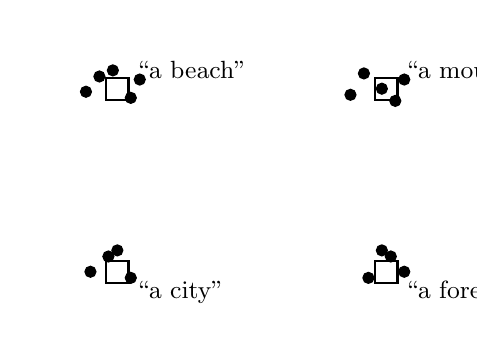
\begin{tikzpicture}
    \begin{axis}[
        xlabel={}, ylabel={},
        xmin=0, xmax=10, ymin=0, ymax=10,
        width=0.6\textwidth, height=0.45\textwidth,
        axis line style={draw=none},
        tick style={black, thin},
        xtick=\empty, ytick=\empty,
    ]
    % Image embeddings: four loose clusters of photo dots
    \addplot[only marks, mark=*, mark size=2pt, black] coordinates {
        (1.6, 8.4) (2.3, 7.7) (1.9, 8.6) (1.3, 7.9) (2.5, 8.3)
    };
    \addplot[only marks, mark=*, mark size=2pt, black] coordinates {
        (7.5, 8.5) (8.2, 7.6) (7.9, 8.0) (8.4, 8.3) (7.2, 7.8)
    };
    \addplot[only marks, mark=*, mark size=2pt, black] coordinates {
        (1.8, 2.5) (2.3, 1.8) (1.4, 2.0) (2.0, 2.7)
    };
    \addplot[only marks, mark=*, mark size=2pt, black] coordinates {
        (8.1, 2.5) (7.6, 1.8) (8.4, 2.0) (7.9, 2.7)
    };
    % Text-prompt anchors as open squares
    \addplot[only marks, mark=square, mark size=4pt, black, thick] coordinates {
        (2.0, 8.0) (8.0, 8.0) (2.0, 2.0) (8.0, 2.0)
    };
    \node[font=\small, anchor=south west] at (axis cs:2.2, 8.0) {``a beach''};
    \node[font=\small, anchor=south west] at (axis cs:8.2, 8.0) {``a mountain''};
    \node[font=\small, anchor=north west] at (axis cs:2.2, 2.0) {``a city''};
    \node[font=\small, anchor=north west] at (axis cs:8.2, 2.0) {``a forest''};
    \end{axis}
\end{tikzpicture}
\caption{A shared embedding space. Image embeddings (filled dots) and text-prompt embeddings (open squares) live in the same space; the predicted class for each photo is the nearest prompt. The encoder was never trained on these specific photos or these specific class names.}
\label{fig:transfer_intro_embedding}
\end{figure}

\marginnote{
\begin{itemize}
    \item How does the model classify your photos if it never saw them?
    \item What does ``knowing what a beach is'' mean for an encoder?
    \item Why might the same trick fail if the four classes were ``part A'', ``part B'', ``part C'', and ``part D'' from a factory line?
\end{itemize}}

\newthought{The model never saw your photos.} It was trained on hundreds of millions of image-caption pairs scraped from the web, none of them labelled with beach, mountain, city, or forest. Yet it can place your photos and your class names into a shared embedding space where similarity does the classification for you, because the words and images that produced its training data already covered most of what your photos contain.

\newthought{From-scratch training would refuse this scenario.} With two hundred unlabelled photos and four target classes, a network trained from scratch has no signal at all, and even with labels two hundred examples sit far below the threshold where a deep model finds anything that generalises. The clustering methods of Part~I would group photos by colour and texture but cannot tell which group is the beach.

\newthought{Reuse changes the question.} The encoder has already done the heavy lifting on someone else's data. You inherit a feature space that knows what beaches and mountains look like, and your job shrinks to writing the right text prompt. The chapter develops the mechanism of reuse from this starting point, through the pretrained backbone you freeze and probe, to the foundation model you query in natural language.

\begin{marginfigure}
\centering
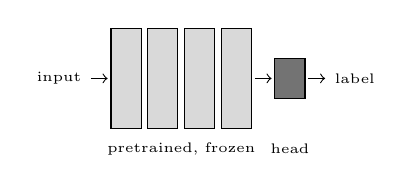
\begin{tikzpicture}[scale=0.85]
    % Pretrained, frozen backbone: four light blocks
    \draw[fill=black!15, draw=black] (0.0,0) rectangle (0.45,1.5);
    \draw[fill=black!15, draw=black] (0.55,0) rectangle (1.0,1.5);
    \draw[fill=black!15, draw=black] (1.1,0) rectangle (1.55,1.5);
    \draw[fill=black!15, draw=black] (1.65,0) rectangle (2.1,1.5);
    \node[font=\tiny] at (1.05,-0.3) {pretrained, frozen};
    % Trainable head: dark block
    \draw[fill=black!55, draw=black] (2.45,0.45) rectangle (2.9,1.05);
    \node[font=\tiny] at (2.675,-0.3) {head};
    % Forward arrows
    \draw[->, thin] (-0.3,0.75) -- (-0.05,0.75);
    \draw[->, thin] (2.15,0.75) -- (2.4,0.75);
    \draw[->, thin] (2.95,0.75) -- (3.2,0.75);
    \node[font=\tiny, anchor=east] at (-0.3,0.75) {input};
    \node[font=\tiny, anchor=west] at (3.2,0.75) {label};
\end{tikzpicture}
\caption{The signature operation of transfer learning: a pretrained backbone is frozen and a small head is trained on top. Most of the chapter is variations on what to freeze, what to adapt, and how cheaply.}
\label{fig:transfer_signature}
\end{marginfigure}

\marginnote{\newthought{Pretraining as infrastructure.} Backbones are starting to look less like models you train and more like libraries you import. The encoder is built once at great cost and used many times at low cost, the same shape as compilers, operating systems, and standard libraries before it.}

\newthought{The Learning Objectives} of this lecture:
\begin{itemize}
    \item Understand backbones, foundation models, and how they emerge from large-scale pretraining.
    \item Apply transfer strategies along a continuum, from frozen feature extraction and linear probing through fine-tuning, parameter-efficient adaptation, and prompting, and pick the right strategy by data regime and domain gap.
    \item Identify when zero-shot and few-shot approaches are appropriate, and diagnose when transfer fails because of distribution shift or negative transfer.
\end{itemize}




%═══════════════════════════════════════════════════════════════════════
% BLOCK 2: MAIN THEORY
%═══════════════════════════════════════════════════════════════════════

%───────────────────────────────────────────────────────────────────────
% SECTION 1: Embeddings, Backbones, Foundation Models
%───────────────────────────────────────────────────────────────────────

\newpage
\section{Embeddings, Backbones, Foundation Models}\index{embedding}\index{backbone}\index{foundation model}

\marginnote{\newthought{The asset is the encoder.} Everything else, the data loader, the loss function, the optimisation schedule, exists to produce one thing: an encoder whose embeddings are worth reusing.}

\newthought{An embedding} is a learned mapping from raw inputs to a vector space where geometry carries meaning. We met this idea in Chapter~6 with the autoencoder and the variational autoencoder. A high-dimensional input was compressed through a bottleneck, and the resulting low-dimensional code retained what the data had in common while discarding what it did not. The decoder was needed for training, but once training had finished, the encoder by itself was already a tool, a fixed function from inputs to a feature space where similarity, classification, and clustering all become easier than in the raw input.

\newthought{What makes that encoder reusable} is the bottleneck argument from Chapter~6. A $k$-dimensional embedding with $k \ll d$ cannot memorise its inputs. It has to throw away the noise and keep what generalises across examples, which is precisely the content that any downstream model needs in order to perform well on new inputs. The encoder that does this well for one corpus tends to do it well for many, and the rest of this chapter is the consequence.

\subsection{Origin: From Hand-Crafted Features to ImageNet Pretraining}

\marginnote{\newthought{Pre-2012 vision} ran on hand-engineered features such as SIFT, HOG, SURF, and GIST. Each was a clever description of edges or gradients designed by humans. They worked, they were the state of the art for a decade, but they did not learn.}

\newthought{The reuse story} did not start with deep learning. Computer vision has lived on shared feature extractors since the 2000s. SIFT, HOG, and their cousins were hand-engineered front ends that the entire field used in common, with task-specific classifiers bolted on top. The pattern was already there: build the encoder once, share it everywhere. What was missing was a way to learn the encoder from data instead of writing it down by hand.

\newthought{What changed in 2012} was the source of the encoder. AlexNet\cite{Krizhevsky2012} was trained end-to-end on ImageNet and won that year's classification benchmark by a wide margin. Within two years it became clear that the network's penultimate layer was, in itself, a better feature extractor than any hand-engineered alternative for almost every other vision task. Razavian et al.\cite{Razavian2014} captured the lesson in a paper title that became a slogan: CNN features off-the-shelf, an astounding baseline. Yosinski et al.\cite{Yosinski2014} quantified which layers transferred, finding that early layers were generic across tasks while late layers were tied to the source objective.

\newthought{The lesson generalised quickly.} Once the field had one example of a network whose features were useful for everything else, it produced many more. ResNet, VGG, Inception, and later vision transformers\cite{Dosovitskiy2020ViT} all became standard backbones, distributed as pretrained weights and reused by the rest of the field. Backbones became infrastructure in the same sense that compilers and operating systems are infrastructure: built once at great cost, used many times at low cost.

\subsection{Backbones, Defined}

\newthought{A backbone}\index{backbone} is a pretrained encoder reused as a feature extractor. The two qualifiers matter. ``Pretrained'' means someone else paid for the training, on a different dataset, for a different objective. ``Reused'' means the encoder is treated as a fixed asset, plugged into a new pipeline whose only job is to produce the task-specific output on top.

\begin{figure}
\centering
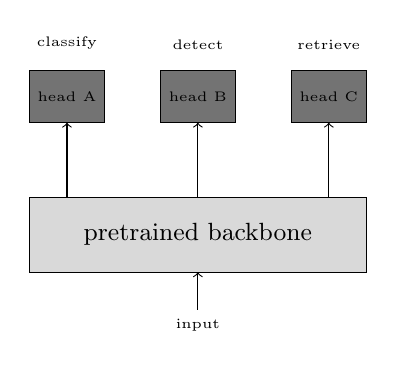
\begin{tikzpicture}[scale=0.95]
    % Single backbone at the bottom
    \draw[fill=black!15, draw=black] (1.0,0) rectangle (5.5,1.0);
    \node[font=\small] at (3.25,0.5) {pretrained backbone};
    % Three heads
    \draw[fill=black!55, draw=black] (1.0,2.0) rectangle (2.0,2.7);
    \node[font=\tiny] at (1.5,2.35) {head A};
    \draw[fill=black!55, draw=black] (2.75,2.0) rectangle (3.75,2.7);
    \node[font=\tiny] at (3.25,2.35) {head B};
    \draw[fill=black!55, draw=black] (4.5,2.0) rectangle (5.5,2.7);
    \node[font=\tiny] at (5.0,2.35) {head C};
    % Arrows up
    \draw[->, thin] (1.5,1.0) -- (1.5,2.0);
    \draw[->, thin] (3.25,1.0) -- (3.25,2.0);
    \draw[->, thin] (5.0,1.0) -- (5.0,2.0);
    % Output labels
    \node[font=\tiny, anchor=south] at (1.5,2.85) {classify};
    \node[font=\tiny, anchor=south] at (3.25,2.85) {detect};
    \node[font=\tiny, anchor=south] at (5.0,2.85) {retrieve};
    % Input arrow at bottom
    \draw[->, thin] (3.25,-0.5) -- (3.25,0);
    \node[font=\tiny, anchor=north] at (3.25,-0.5) {input};
\end{tikzpicture}
\caption{One backbone, many heads. The encoder is trained once on a broad pretraining task and serves as the input stage for many downstream tasks. The cost of the encoder is amortised across every task that shares it.}
\label{fig:backbone_many_heads}
\end{figure}

\begin{marginfigure}
\centering
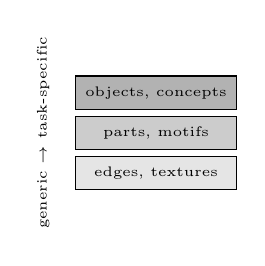
\begin{tikzpicture}[scale=0.85]
    \draw[fill=black!10, draw=black] (0,0) rectangle (2.4,0.5);
    \node[font=\tiny] at (1.2,0.25) {edges, textures};
    \draw[fill=black!20, draw=black] (0,0.6) rectangle (2.4,1.1);
    \node[font=\tiny] at (1.2,0.85) {parts, motifs};
    \draw[fill=black!30, draw=black] (0,1.2) rectangle (2.4,1.7);
    \node[font=\tiny] at (1.2,1.45) {objects, concepts};
    \node[font=\tiny, rotate=90, anchor=south] at (-0.25,0.85) {generic $\to$ task-specific};
\end{tikzpicture}
\caption{What each layer learns and how transferable it is. Early layers capture edges and textures generic across tasks; late layers capture concepts tied to the source task. The reuse strategies in Section~2 trade off these axes.}
\label{fig:layer_hierarchy}
\end{marginfigure}

\newthought{Figure~\ref{fig:backbone_many_heads} is not a piece of architecture}, it is a piece of economics. Training the backbone is the expensive operation, paid for once. Each head is a small classifier or regressor that adapts the backbone's output to a specific task and is trained on a task-specific dataset that may be tiny. The backbone never sees the task-specific data while it is being built; the task-specific data never pays the cost of pretraining.

\newthought{Generalisation}\index{generalisation} is the reason this works. A bottlenecked encoder must compress, and compression requires ignoring idiosyncratic noise in favour of shared structure. A $k$-dimensional embedding with $k \ll d$ cannot memorise individual inputs; it must discover regularities that hold across the training distribution. Those regularities, the semantic features, are precisely what a downstream model needs to perform well on data it never saw during training.

\subsection{Pretraining Datasets}

\newthought{Where the backbone comes from} is the design decision that matters most at this stage. The encoder is only as general as the data it was trained on, and across domains a small number of large-scale datasets have become the standard foundations for pretraining. Each engraves its own statistical fingerprint into every backbone built on top of it.

\begin{table*}[ht]
\centering
\begin{tabular}{p{0.14\textwidth}p{0.10\textwidth}p{0.10\textwidth}p{0.38\textwidth}}
    \toprule
    \textbf{Dataset} & \textbf{Modality} & \textbf{Scale} & \textbf{What the backbone learns} \\
    \midrule
    ImageNet \citealt{Deng2009ImageNet} & Images & 14M images & Edges, textures, object parts, and category-level semantics. The de facto starting point for visual feature extractors. \\
    The Pile \citealt{Gao2020Pile} & Text & 825 GB text & Syntax, coreference, factual associations, and discourse structure from books, academic papers, web text, and code. \\
    LibriSpeech \citealt{Panayotov2015LibriSpeech} & Audio & 1000 h audio & Phoneme boundaries, prosody, and speaker-invariant representations from read English speech. \\
    Kinetics-700 \citealt{Carreira2022Kinetics700} & Video & 650k clips & Temporal dynamics, motion patterns, and action semantics from short video clips spanning 700 human action classes. \\
    ShapeNet \citealt{Chang2015ShapeNet} & 3D shapes & 51k models & Surface geometry, part decomposition, and pose-invariant structure from annotated CAD models across 55 object categories. \\
    LAION-5B \citealt{Schuhmann2022LAION5B} & Image + text & 5.8B pairs & Joint visual and linguistic semantics from web-crawled image-caption pairs; the foundation behind open multimodal models. \\
    CheXpert \citealt{Irvin2019CheXpert} & Medical images & 224k X-rays & Anatomical landmarks, pathology signatures, and radiological texture patterns from labelled chest radiographs. \\
    ZINC \citealt{Sterling2015ZINC} & Molecular graphs & 250k molecules & Bond topology, functional-group motifs, and drug-likeness features from curated small-molecule structures. \\
    \bottomrule
\end{tabular}
\vspace{2em}
\caption{Large-scale pretraining datasets across modalities. Each dataset supplies the raw material for a backbone to learn general-purpose features that transfer to downstream tasks within and sometimes across its modality.}
\label{tab:pretraining_datasets}
\end{table*}

\marginnote{\newthought{Modality matters.} An ImageNet backbone transfers well to satellite imagery or medical photos, but poorly to molecular graphs or audio spectrograms. Choosing the right source dataset and modality is the first design decision in any transfer learning pipeline.}

\subsection{Foundation Models}\index{foundation model}

\marginnote{\newthought{The term} was coined by the Stanford CRFM group\cite{Bommasani2021Foundation}. It is contested, but the phenomenon it names is real: a single pretrained model that serves dozens of downstream tasks without further training.}

\newthought{Foundation models} are backbones at a different scale. The data is broader, the parameters are larger, and the training compute is larger still. The architecture is rarely new. What is new is what the backbone has seen and how much of it. CLIP\cite{Radford2021CLIP} saw four hundred million image-caption pairs scraped from the web. GPT-style language models\cite{Brown2020GPT3} saw most of the internet's text. SAM\cite{Kirillov2023SAM} saw a billion segmentation masks. The result is a backbone whose embeddings cover so much of the world that many tasks can be solved without any task-specific training, by querying the pretrained model directly.

\newthought{The third ingredient,} on top of scale and breadth, is alignment across modalities. CLIP's two encoders were trained jointly so that an image of a dog and the text ``a photo of a dog'' land near each other in a shared embedding space. The alignment is the bridge that turns a vision encoder into a zero-shot classifier in Section~3, and it is what separates a foundation model from an ordinary backbone in practice.

\newthought{Notice that a foundation model is just a backbone} with three additions: bigger, broader, and often cross-modal. There is no new architecture, no new layer type, no new optimiser. The leap is quantitative on every axis except one, and the qualitative consequence, emergent zero-shot capability, falls out of those quantitative differences. The remaining sections of this chapter work out how.

\vspace{2.5em}

%───────────────────────────────────────────────────────────────────────
% SECTION 2: The Transfer Continuum
%───────────────────────────────────────────────────────────────────────

\newpage
\section{The Transfer Continuum}\index{transfer learning}\index{fine-tuning}

\marginnote{\newthought{What to freeze, what to train.} Every transfer technique answers the same two questions, which parameters move during adaptation, and how much target supervision is required to move them. Different answers sit at different points on a continuum.}

\newthought{Section~1 asked where backbones come from.} This section asks how to use one. The choice is not binary, freeze or retrain, but a continuum of techniques that trade two costs against each other: how much of the backbone you are willing to update, and how much labelled target data you are willing to spend updating it. At one extreme you change nothing and pay nothing in target labels. At the other you retrain the whole backbone and need a lot of target data. Most real projects sit somewhere between, and the rest of this section maps the space.

\begin{figure}
\centering
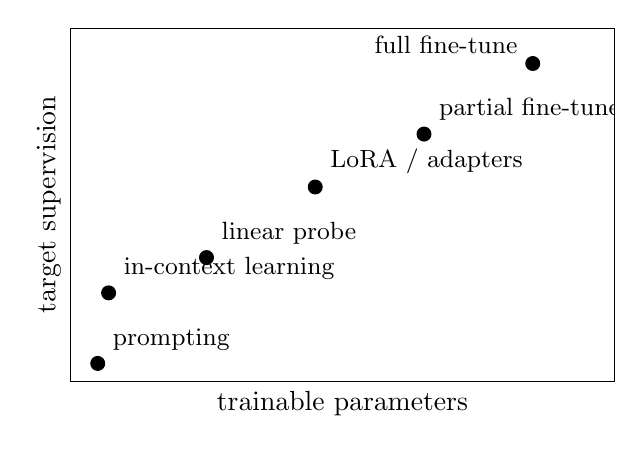
\begin{tikzpicture}
    \begin{axis}[
        xlabel={trainable parameters},
        ylabel={target supervision},
        xmin=0, xmax=10, ymin=0, ymax=10,
        width=0.7\textwidth, height=0.5\textwidth,
        axis line style={black, thin},
        tick style={black, thin},
        xtick=\empty, ytick=\empty,
        xlabel near ticks, ylabel near ticks,
    ]
    \addplot[only marks, mark=*, mark size=2.5pt, black] coordinates {(0.5, 0.5)};
    \node[font=\small, anchor=south west] at (axis cs:0.6, 0.6) {prompting};
    \addplot[only marks, mark=*, mark size=2.5pt, black] coordinates {(0.7, 2.5)};
    \node[font=\small, anchor=south west] at (axis cs:0.8, 2.6) {in-context learning};
    \addplot[only marks, mark=*, mark size=2.5pt, black] coordinates {(2.5, 3.5)};
    \node[font=\small, anchor=south west] at (axis cs:2.6, 3.6) {linear probe};
    \addplot[only marks, mark=*, mark size=2.5pt, black] coordinates {(4.5, 5.5)};
    \node[font=\small, anchor=south west] at (axis cs:4.6, 5.6) {LoRA / adapters};
    \addplot[only marks, mark=*, mark size=2.5pt, black] coordinates {(6.5, 7.0)};
    \node[font=\small, anchor=south west] at (axis cs:6.6, 7.1) {partial fine-tune};
    \addplot[only marks, mark=*, mark size=2.5pt, black] coordinates {(8.5, 9.0)};
    \node[font=\small, anchor=south east] at (axis cs:8.4, 9.0) {full fine-tune};
    \end{axis}
\end{tikzpicture}
\caption{The transfer continuum. Each strategy occupies a position in the plane of trainable parameters against required target supervision. Cheaper strategies sit at the bottom-left and rely almost entirely on the backbone; more expensive strategies sit at the top-right and trade target labels for adaptability.}
\label{fig:transfer_continuum}
\end{figure}

\subsection{Frozen Features and Linear Probing}\index{linear probe}

\newthought{The cheapest reuse strategy} is to freeze the backbone entirely and use it once. Feed every input through the encoder, store the resulting embeddings, and train a small classifier on those embeddings. The backbone is computed once per input, never updated, and the only training loop runs over the classifier on top.

\newthought{Linear probing} is the canonical version. Freeze the encoder $f_\theta$ and train a single linear layer $W$ on top, optimising
\begin{align*}
    \min_{W} \sum_i \mathcal{L}\bigl(W^\top f_\theta(x_i),\, y_i\bigr).
\end{align*}
The objective has the same shape as logistic regression on hand-engineered features, except the features now come from a deep encoder. With a strong backbone, linear probing is often within a few points of full fine-tuning, at a small fraction of the cost.

\marginnote{\newthought{Linear-probe protocol.} Compute embeddings once, cache them, sweep regularisation strengths on the cached vectors, pick by validation accuracy. The whole loop runs on a laptop even when the backbone needed a cluster to train.}

\newthought{Linear probing is also the standard diagnostic} for backbone quality. A new self-supervised method or a new pretraining dataset is almost always evaluated by reporting linear-probe accuracy on a fixed downstream benchmark, because the result isolates the encoder's contribution from the classifier's expressiveness. If the linear probe does well, the encoder is good; if it does badly, no amount of head engineering will rescue it.

\subsection{Fine-Tuning}\index{fine-tuning}

\newthought{When source and target domains differ enough} that frozen features are insufficient, the next step is to update some or all of the backbone's parameters. Fine-tuning unfreezes a chosen set of layers and trains them on the target data, typically with a much smaller learning rate than the original pretraining used.

\newthought{Partial fine-tuning} unfreezes only the late layers, leaving early layers untouched. This follows the layer-hierarchy logic of Section~1: early layers encode features that are generic across domains, so they rarely benefit from adaptation, while late layers encode task-specific concepts that often do. The learning-rate schedule frequently mirrors this, with later layers receiving larger updates than earlier ones.

\newthought{Full fine-tuning} unfreezes everything. It is the most flexible and the most expensive, both in compute and in target labels, and it carries the largest risk of catastrophic forgetting.

\marginnote{\newthought{Catastrophic forgetting.}\index{catastrophic forgetting} A network that fine-tunes aggressively on a small target dataset can lose its ability to perform the source task. The encoder's earlier knowledge is overwritten by gradient updates that optimise only the new objective. Lower learning rates, fewer epochs, layer-wise learning-rate decay, and replay of source examples all reduce the damage.}

\subsection{Parameter-Efficient Fine-Tuning}\index{PEFT}\index{LoRA}

\newthought{Full fine-tuning becomes impractical} once a backbone has billions of parameters. Storing one optimiser state per parameter, updating each weight, and saving a separate checkpoint per downstream task all scale with model size, and at modern scale none of them is cheap. Parameter-efficient fine-tuning, or PEFT, freezes the backbone and adds a small number of trainable parameters elsewhere, in such a way that the original weights are recovered when the new parameters are zero.

\newthought{LoRA}\cite{Hu2021LoRA} is the dominant PEFT technique. Leave the backbone weights $W$ frozen and represent the update $\Delta W$ as a low-rank matrix product:
\begin{align*}
    W_{\text{adapted}} &= W + \Delta W, \\
    \Delta W &= B A,
\end{align*}
where $A \in \mathbb{R}^{r \times d_{\text{in}}}$ and $B \in \mathbb{R}^{d_{\text{out}} \times r}$ with $r \ll \min(d_{\text{in}}, d_{\text{out}})$. Only $A$ and $B$ are trained, so the trainable parameter count drops from $d_{\text{in}} d_{\text{out}}$ to $r(d_{\text{in}}{+}d_{\text{out}})$. For a 7B-parameter language model and rank $r{=}8$, the LoRA adapters add a few tens of megabytes against a backbone that occupies tens of gigabytes.

\begin{marginfigure}
\centering
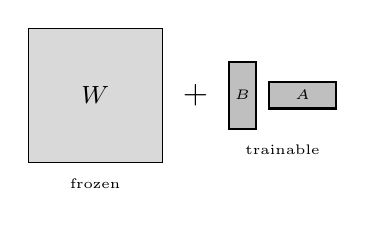
\begin{tikzpicture}[scale=0.85]
    \draw[fill=black!15, draw=black] (0,0) rectangle (2.0, 2.0);
    \node[font=\small] at (1.0, 1.0) {$W$};
    \node[font=\tiny, anchor=north] at (1.0, -0.1) {frozen};
    \node[font=\large] at (2.5, 1.0) {$+$};
    \draw[fill=black!25, draw=black, thick] (3.0, 0.5) rectangle (3.4, 1.5);
    \node[font=\tiny] at (3.2, 1.0) {$B$};
    \draw[fill=black!25, draw=black, thick] (3.6, 0.8) rectangle (4.6, 1.2);
    \node[font=\tiny] at (4.1, 1.0) {$A$};
    \node[font=\tiny, anchor=north] at (3.8, 0.4) {trainable};
\end{tikzpicture}
\caption{LoRA freezes the original weight matrix $W$ and adds a low-rank update $BA$. The product has the same shape as $W$ but only $r(d_{\text{in}}{+}d_{\text{out}})$ trainable parameters.}
\label{fig:lora}
\end{marginfigure}

\marginnote{\newthought{PEFT siblings.} Adapters\cite{Houlsby2019Adapters} insert small bottleneck layers between transformer blocks. BitFit\cite{ZakenBitFit2022} fine-tunes only the bias terms. Prompt tuning learns a soft prompt of trainable token embeddings prepended to the input. Each occupies a different point on the parameter-cost-versus-flexibility trade-off, and LoRA happens to be the most popular because it preserves inference latency.}

\newthought{The deeper consequence} is that adaptation becomes composable. A single frozen backbone can serve many tasks, each with its own small LoRA adapter swapped in at inference time. The economics of Section~1 reappears: the backbone is the asset, the adapters are cheap task-specific extensions, and many of them coexist on top of one shared encoder.

\subsection{Prompting and In-Context Learning}\index{prompt engineering}\index{in-context learning}

\newthought{The extreme parameter-efficient case} is to train no parameters at all. Some foundation models, especially large language models, can be steered by the input alone, without any gradient updates. The control surface is the prompt, the text or other input that precedes the actual query and conditions the model's behaviour on it.

\newthought{Zero-shot prompting} sends only the task description, for example, ``Classify the following review as positive or negative. Review: \ldots''. In-context learning\index{ICL} sends a handful of input-output pairs alongside the description, before the actual query, and the model imitates the pattern. No weights move, no gradients flow, and yet the output adapts to the examples it just saw.

\marginnote{\newthought{ICL details} belong to the upcoming lecture series on large language models. Here ICL is just the no-gradient endpoint of the transfer continuum, the smallest possible parameter cost, paid in prompt tokens instead of weight updates.}

\newthought{Prompting is parameter-free} but it is not free. Each example added to the prompt increases the input length, which costs compute and latency at inference, and the prompt has to fit within the model's context window. Prompt engineering, the discipline of writing prompts that get the desired behaviour, becomes a real engineering practice, with template libraries, ablation studies, and structured outputs as standard tools.

\subsection{Choosing a Strategy}

\marginnote{\newthought{Recipe.} The table below is a starting point, not a law. Real projects iterate, often starting at the cheap end and moving rightwards on the continuum only when the cheaper option is shown to be insufficient.}

\newthought{The continuum yields a recipe.} Pick the cheapest strategy that meets the target accuracy, and only pay for more parameters when the cheaper option provably falls short.

\begin{table*}[ht]
\centering
\begin{tabular}{p{0.18\textwidth}p{0.16\textwidth}p{0.14\textwidth}p{0.34\textwidth}}
    \toprule
    \textbf{Target labels} & \textbf{Domain gap} & \textbf{Strategy} & \textbf{Why} \\
    \midrule
    Zero & Small & Zero-shot prompting & The backbone already covers the target task; describe the task in text and read the answer. \\
    A few examples & Small & In-context learning & Show the model the pattern in the prompt; no training needed. \\
    Tens to hundreds & Small & Linear probe & Frozen embeddings plus a single linear layer, cheap and reproducible. \\
    Hundreds to thousands & Medium & LoRA / adapter & Update a small number of parameters and preserve the backbone for other tasks. \\
    Thousands or more & Medium to large & Partial fine-tuning & Adapt the late layers where task specificity lives. \\
    Many thousands or more & Large & Full fine-tuning & Update everything, accept the catastrophic-forgetting risk, and budget for compute. \\
    \bottomrule
\end{tabular}
\vspace{2em}
\caption{A starting recipe for choosing a transfer strategy. Move down the table as the domain gap and the volume of available target labels grow.}
\label{tab:transfer_recipe}
\end{table*}

\newthought{Notice that the ordering} is by parameter cost, not by accuracy. A linear probe on a strong backbone often beats full fine-tuning on a weak one, especially when target data is scarce. The right question is rarely which strategy is most powerful, but which strategy makes the best use of the labels and compute on hand.

\subsection{When Transfer Fails}\index{negative transfer}

\marginnote{\newthought{Failure mode.} Transfer is not a free lunch. The backbone supplies a strong inductive bias, and when that bias is wrong for the target task, transfer hurts.}

\newthought{Negative transfer} is the case where reusing a pretrained backbone produces lower accuracy than training from scratch would. It happens when the source and target distributions are far enough apart that the backbone's features are actively misleading rather than merely uninformative. An ImageNet backbone applied to molecular graphs, a language model fine-tuned on legal documents that drifts toward casual web tone, or a satellite-imagery encoder pulled into medical X-rays all illustrate the same failure: the backbone's prior fights the target objective instead of helping it.

\newthought{Catastrophic forgetting} is the related failure of fine-tuning. When the model is updated on the target task with a learning rate that is too aggressive, or for too many epochs, the original capabilities are overwritten by gradient updates whose only signal is the new objective. The model becomes good at the target task and bad at everything else, which is a problem when ``everything else'' was the reason the backbone was useful in the first place.

\newthought{Distribution shift} is the operational version of negative transfer.\index{distribution shift} The model was trained on one distribution and is deployed on another, and the gap between the two erodes performance silently. Three flavours recur. Covariate shift\index{covariate shift} occurs when $P(X)$ changes but $P(Y \mid X)$ stays the same: the inputs look different but the labelling rule is unchanged. Label shift\index{label shift} occurs when $P(Y)$ changes but $P(X \mid Y)$ stays the same: class proportions move but each class still produces the same kind of inputs. Concept drift\index{concept drift} occurs when $P(Y \mid X)$ changes over time: the same input now carries a different label, often because the world has changed.

\marginnote{\newthought{Adversarial domain adaptation}\cite{Ganin2016DomainAdversarial} learns features that are informative for the task but indistinguishable across domains, by training a domain discriminator and asking the encoder to fool it. The technique is a clean instance of the broader pattern, learn invariances explicitly when the data does not supply them.}

\newthought{The remedies for each shift type} differ. Covariate shift is often addressed by importance weighting or by domain adaptation. Label shift can be corrected analytically when the new class proportions are known. Concept drift typically requires retraining, with the harder challenge of detecting the drift before the model is already wrong. Chapter~7 supplies the operational tools, calibration, OOD detection, and monitoring, that catch these failures in deployment, and this chapter supplies the adaptation techniques that respond to them.

\vspace{2.5em}

%═══════════════════════════════════════════════════════════════════════
% SECTION 3 PLACEHOLDER (Zero- and Few-Shot Learning)
% Replace from PLACEHOLDER START to PLACEHOLDER END (markers inclusive)
% with the full Section 3 draft. Scope in the chapter scope scaffold at
% the top of this file. Includes the LLM-prompting thumbnail thread.
%═══════════════════════════════════════════════════════════════════════

% >>>>>>>>>>>>>>>> SECTION 3 PLACEHOLDER START <<<<<<<<<<<<<<<<

\newpage
\section{Zero- and Few-Shot Learning}\index{zero-shot learning}\index{few-shot learning}

\marginnote{\newthought{Zero examples, one example, a handful.} Section~2 mapped strategies by how many parameters they update. Here we map them by how many target-class examples they need. The two axes meet at the bottom-left corner: zero parameters and zero examples, the regime that used to be impossible.}

\newthought{Section~2 ended with a recipe} that ranges from full fine-tuning to prompting, ordered by how much of the backbone is allowed to move. The cheap end of that continuum, prompting and in-context learning, is also the regime where target labels are scarcest. This section follows the cheap end into its sharpest form: classifying with no labelled examples at all, or with a handful, by leaning entirely on a backbone that already knows enough about the world to recognise the new task when it sees it.

\subsection{Origin: Attribute-Based Zero-Shot}\index{attribute-based zero-shot}

\marginnote{\newthought{The bridge problem.} Zero-shot classification needs some link between class semantics and image features. Without examples of the new class, the link cannot be learned from data; it has to come from somewhere else. Pre-2020 it came from a hand-built table.}

\newthought{The first formulation of zero-shot} classification in computer vision came from Lampert and colleagues in 2009\cite{Lampert2009}. They asked a simple question: can a model classify an animal it has never seen during training, given only a description of what that animal looks like? Their answer was a hand-built class-attribute table. Each class, seen or unseen, was encoded as a vector of binary attributes such as striped, four-legged, mammal, lives-in-water. A zebra became striped + four-legged + mammal + black-and-white; a dolphin became smooth + lives-in-water + mammal.

\newthought{The model was not trained on classes,} it was trained on attributes. Each attribute had its own classifier, trained on whichever seen classes had that attribute. At inference time, an image was passed through every attribute classifier, the outputs were assembled into a predicted attribute vector, and the image was assigned to the class whose attribute vector lay closest. The unseen classes had never produced a single training image, but their attribute descriptions slotted into the same table as the seen classes, so the comparison was well defined.

\newthought{The lesson outlasted the method.} Zero-shot classification needs a bridge between class semantics and image features, and the bridge has to come from outside the labelled training set. Lampert's bridge was a hand-curated attribute ontology, which is expensive to build, narrow in coverage, and hard to extend. The structural insight, that an external semantic representation of the target classes is what makes zero-shot possible, survived long after the table-of-attributes implementation was abandoned.

\begin{figure}
\centering
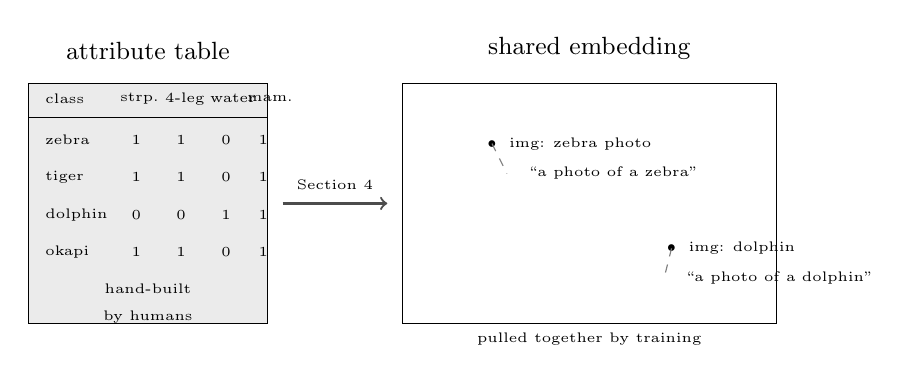
\begin{tikzpicture}[scale=0.95]
    % LEFT: Lampert attribute table
    \node[font=\small, anchor=south] at (1.6, 3.4) {attribute table};
    \draw[fill=black!8, draw=black] (0.0, 0.0) rectangle (3.2, 3.2);
    \node[font=\tiny, anchor=west] at (0.1, 3.0) {class};
    \node[font=\tiny, anchor=west] at (1.1, 3.0) {strp.};
    \node[font=\tiny, anchor=west] at (1.7, 3.0) {4-leg};
    \node[font=\tiny, anchor=west] at (2.3, 3.0) {water};
    \node[font=\tiny, anchor=west] at (2.8, 3.0) {mam.};
    \draw[black, thin] (0.0, 2.75) -- (3.2, 2.75);
    \node[font=\tiny, anchor=west] at (0.1, 2.45) {zebra};
    \node[font=\tiny, anchor=west] at (1.25, 2.45) {1};
    \node[font=\tiny, anchor=west] at (1.85, 2.45) {1};
    \node[font=\tiny, anchor=west] at (2.45, 2.45) {0};
    \node[font=\tiny, anchor=west] at (2.95, 2.45) {1};
    \node[font=\tiny, anchor=west] at (0.1, 1.95) {tiger};
    \node[font=\tiny, anchor=west] at (1.25, 1.95) {1};
    \node[font=\tiny, anchor=west] at (1.85, 1.95) {1};
    \node[font=\tiny, anchor=west] at (2.45, 1.95) {0};
    \node[font=\tiny, anchor=west] at (2.95, 1.95) {1};
    \node[font=\tiny, anchor=west] at (0.1, 1.45) {dolphin};
    \node[font=\tiny, anchor=west] at (1.25, 1.45) {0};
    \node[font=\tiny, anchor=west] at (1.85, 1.45) {0};
    \node[font=\tiny, anchor=west] at (2.45, 1.45) {1};
    \node[font=\tiny, anchor=west] at (2.95, 1.45) {1};
    \node[font=\tiny, anchor=west] at (0.1, 0.95) {okapi};
    \node[font=\tiny, anchor=west] at (1.25, 0.95) {1};
    \node[font=\tiny, anchor=west] at (1.85, 0.95) {1};
    \node[font=\tiny, anchor=west] at (2.45, 0.95) {0};
    \node[font=\tiny, anchor=west] at (2.95, 0.95) {1};
    \node[font=\tiny, anchor=north] at (1.6, 0.65) {hand-built};
    \node[font=\tiny, anchor=north] at (1.6, 0.30) {by humans};
    % RIGHT: cross-modal embedding space
    \node[font=\small, anchor=south] at (7.5, 3.4) {shared embedding};
    \draw[black, thin] (5.0, 0.0) rectangle (10.0, 3.2);
    \node[font=\tiny] at (6.2, 2.4) {$\bullet$};
    \node[font=\tiny, anchor=west] at (6.3, 2.4) {img: zebra photo};
    \node[font=\tiny] at (6.4, 2.0) {$\square$};
    \node[font=\tiny, anchor=west] at (6.55, 2.0) {``a photo of a zebra''};
    \node[font=\tiny] at (8.6, 1.0) {$\bullet$};
    \node[font=\tiny, anchor=west] at (8.7, 1.0) {img: dolphin};
    \node[font=\tiny] at (8.5, 0.6) {$\square$};
    \node[font=\tiny, anchor=west] at (8.65, 0.6) {``a photo of a dolphin''};
    \draw[black!50, dashed, thin] (6.2, 2.4) -- (6.4, 2.0);
    \draw[black!50, dashed, thin] (8.6, 1.0) -- (8.5, 0.6);
    \node[font=\tiny, anchor=north] at (7.5, 0.0) {pulled together by training};
    % Arrow connecting the two
    \draw[->, thick, black!70] (3.4, 1.6) -- (4.8, 1.6);
    \node[font=\tiny, anchor=south] at (4.1, 1.65) {Section~4};
\end{tikzpicture}
\caption{Two ways to bridge class semantics and image features. On the left, Lampert's attribute table encodes each class as a vector of human-curated attributes; the model classifies images by predicting attributes and matching against the table. On the right, a cross-modal pretraining objective places images and class-name texts into a shared embedding space, so the bridge is built from data instead of by hand.}
\label{fig:lampert_vs_crossmodal}
\end{figure}

\subsection{The Cross-Modal Leap}\index{cross-modal alignment}

\newthought{The bridge that Lampert built by hand} can be built from data, if the data already contains both modalities. The web is full of image-caption pairs, and a model trained to align images with their captions ends up learning, as a side effect, an embedding space where the text ``a photo of a zebra'' and an actual photo of a zebra land near each other. The attribute table is replaced by a text encoder, and the bridge becomes a learned function rather than an authored ontology.

\newthought{Zero-shot classification then collapses to nearest-prompt similarity.} For a target task with classes $\{c_1, \ldots, c_K\}$, each class name is wrapped in a prompt template, embedded by the text encoder, and the predicted class for an image $x$ is
\begin{align*}
    \hat{y} &= \arg\max_{k} \, \cos\bigl(f_{\text{img}}(x),\, f_{\text{txt}}(T(c_k))\bigr),
\end{align*}
where $T$ is a template such as ``a photo of a \{class\}''. There is no training loop, no gradient, no labelled image of the target classes. The classifier is a similarity computation in a space that the backbone built once, on someone else's data.

\newthought{Section~4 will derive this picture in detail} for CLIP, including the contrastive objective that produces the shared space and the diagonal-loss training pattern. For now the picture is enough: the cross-modal pretraining of Section~4 supplies, for free, exactly the bridge that Lampert had to author.

\subsection{Few-Shot Recipes in the Embedding Space}\index{few-shot learning}\index{prototypical networks}

\newthought{When a few labelled examples per class are available,} the same backbone supports a small family of recipes that share a common ingredient: every example, labelled or query, is mapped through the frozen encoder once, and the few-shot logic happens entirely in the embedding space.

\newthought{The linear probe} of Section~2 is the most direct option. Given $K$ shots per class, embed each example with the frozen backbone, and fit a single linear layer on the cached embeddings. With strong backbones and modest $K$ this is often a few accuracy points off full fine-tuning, runs on a laptop, and never touches the backbone weights.

\newthought{Prototypical networks}\cite{Snell2017Prototypical} replace the linear classifier with a centroid. For each class $k$, compute the mean of the few labelled embeddings,
\begin{align*}
    \mu_k &= \tfrac{1}{|S_k|} \sum_{x_i \in S_k} f_\theta(x_i),
\end{align*}
and classify a query $x$ by nearest centroid in the embedding space,
\begin{align*}
    \hat{y} &= \arg\min_k \, \lVert f_\theta(x) - \mu_k \rVert.
\end{align*}
There are no parameters to fit beyond the centroids themselves, and the centroids are computed from the support set in closed form. Nearest-class-mean classification, the same computation under a different name, predates the deep learning era and is the canonical baseline whenever a strong embedding is on hand.

\begin{marginfigure}
\centering
\begin{tikzpicture}
    \begin{axis}[
        xlabel={}, ylabel={},
        xmin=0, xmax=10, ymin=0, ymax=10,
        width=\marginparwidth, height=\marginparwidth,
        axis line style={draw=none},
        tick style={black, thin},
        xtick=\empty, ytick=\empty,
    ]
    % Class A support set + prototype
    \addplot[only marks, mark=*, mark size=2pt, black] coordinates {(1, 2) (2, 3) (3, 1)};
    \addplot[only marks, mark=o, mark size=3pt, black, thick] coordinates {(2, 2)};
    \node[font=\tiny, anchor=west] at (axis cs:2.2, 2.0) {$\mu_A$};
    % Class B support set + prototype
    \addplot[only marks, mark=*, mark size=2pt, black!55] coordinates {(6, 8) (8, 7) (8, 9)};
    \addplot[only marks, mark=o, mark size=3pt, black!55, thick] coordinates {(7.33, 8.0)};
    \node[font=\tiny, anchor=west] at (axis cs:7.5, 8.0) {$\mu_B$};
    % Query point + dashed lines
    \addplot[only marks, mark=x, mark size=3pt, thick, black!30] coordinates {(5, 6)};
    \node[font=\tiny, anchor=north] at (axis cs:5.0, 5.7) {$x$};
    \draw[black!50, dashed, thin] (axis cs:5,6) -- (axis cs:2,2);
    \draw[black!50, dashed, thin] (axis cs:5,6) -- (axis cs:7.33,8.0);
    \end{axis}
\end{tikzpicture}
\caption{A prototypical-networks classifier in the embedding space. Three labelled examples per class produce two prototypes $\mu_A$ and $\mu_B$ as their centroids. The query $x$ is classified by the closer prototype, here $\mu_B$.}
\label{fig:prototypical}
\end{marginfigure}

\newthought{Notice that all three recipes share one ingredient,} the encoder of Section~1 used as a feature extractor. The linear probe, the prototypical network, and the nearest-class-mean classifier differ only in what they do with the resulting embeddings. The heavy lifting is upstream, in the pretraining, and the few-shot stage merely chooses how to convert support embeddings into a decision rule.

\subsection{Prompt Engineering}\index{prompt engineering}

\marginnote{\newthought{Prompt ensembling.} Averaging the text embeddings of dozens of paraphrased prompts smooths over the idiosyncrasy of any single template. The trick is mechanical, the gain is real, and on ImageNet zero-shot it is worth several accuracy points.}

\newthought{The prompt is a hyperparameter.} A zero-shot classifier built from a foundation model is sensitive to how the class names are wrapped in text, because the text encoder produces different embeddings for ``zebra'', ``a photo of a zebra'', and ``a photo of a zebra, a striped african equid''. The first reads as a bare word, the second as a typical caption, and the third supplies the kind of disambiguating context that captions in the training data tended to carry. The third tends to win.

\newthought{Hand-crafted templates} dominate the simplest practice. ``A photo of a \{class\}'' became the de facto baseline because it matches the caption distribution that web-trained models saw most often. Domain-specific templates beat the generic baseline whenever the target task has a recognisable register: ``a satellite photo of \{class\}'' for remote sensing, ``a histopathology slide of \{class\}'' for medical imaging, ``a sketch of \{class\}'' for line art.

\newthought{CoOp}\index{CoOp}\cite{Zhou2022CoOp} replaces the human-written template with learnable token embeddings. The class name is preceded by $M$ continuous vectors $V_1, \ldots, V_M$, optimised on a small labelled set so that the resulting prompt embedding pulls the right images closest. The vectors live in the embedding space, not in the text vocabulary, so the learned ``prompt'' is no longer a sentence; it is a soft prefix that the text encoder reads instead of human language. CoOp routinely beats the best hand-crafted template at the cost of a tiny labelled set and a short training run, and sits squarely in the PEFT corner of the Section~2 continuum.

\subsection{From Prompts to Aligned Models: A Thumbnail}\index{instruction tuning}\index{RLHF}\index{DPO}

\marginnote{\newthought{Thumbnail only.} The full story of large language models, alignment, and reinforcement learning from human feedback belongs to the upcoming LLM lecture series. Here we trace the names of the steps and a one-line framing of each, so that the prompt-engineering beat above lands in its proper place in the timeline.}

\newthought{The prompting story does not end with vision-language models.} Large language models walked their own path from raw prompting to aligned behaviour, and the milestones along the way explain why the prompts a modern student types into a chat interface look almost nothing like what GPT-3 expected. Each step kept the previous one and added a control surface on top.

\newthought{Raw few-shot prompting} was the GPT-3 demonstration\cite{Brown2020GPT3}. A model trained only to predict the next token, with no notion of tasks or instructions, was shown a handful of input-output examples in the prompt and continued the pattern for a new input. Chain-of-thought prompting\cite{Wei2022CoT} added a single rhetorical move, asking the model to think step by step, and unlocked multi-step reasoning that direct prompting could not elicit. Soft prompting and prefix tuning\cite{Lester2021PromptTuning,Li2021PrefixTuning} replaced the human-written prefix with a small set of trainable embeddings, the language analogue of CoOp, and showed that the prompt could itself be learned at a tiny parameter cost. Instruction tuning\cite{Wei2021FLAN,Sanh2021T0} fine-tuned the model on collections of (instruction, response) pairs covering many tasks, so that natural-language instructions, rather than few-shot examples, became the primary control surface. Reinforcement learning from human preferences\cite{Christiano2017Preferences} provided the next layer: humans ranked candidate outputs, a reward model fit those rankings, and the language model was nudged towards preferred behaviour by policy optimisation; InstructGPT\cite{Ouyang2022InstructGPT} brought the recipe to language models at scale and produced the first chat-style assistants. Direct preference optimisation\cite{Rafailov2023DPO} simplified the picture by removing the explicit reward model, treating the language model itself as the reward, and optimising preference data with a single supervised objective.

\newthought{The thread through these steps} is one that this section has already walked in miniature. Each milestone moves the locus of control from the model's weights, to the prompt, and then back into the weights through ever-cheaper supervision: examples in context, learned soft prefixes, instruction-response pairs, ranked preferences, direct preference data. The names matter because they carry the field's vocabulary; the mechanism matters because each one is a way of nudging a backbone whose weights cost too much to retrain. Section~4 returns to vision-language alignment with the contrastive objective that built the embedding space this whole section has stood on.

\vspace{2.5em}

% >>>>>>>>>>>>>>>> SECTION 3 PLACEHOLDER END <<<<<<<<<<<<<<<<


%═══════════════════════════════════════════════════════════════════════
% SECTION 4 PLACEHOLDER (CLIP and Cross-Modal Alignment)
% Replace from PLACEHOLDER START to PLACEHOLDER END (markers inclusive).
%═══════════════════════════════════════════════════════════════════════

% >>>>>>>>>>>>>>>> SECTION 4 PLACEHOLDER START <<<<<<<<<<<<<<<<

\newpage
\section{CLIP and Cross-Modal Alignment [placeholder]}\index{CLIP}\index{cross-modal alignment}

\marginnote{\newthought{Placeholder.} Section~4 will be drafted by a section-drafter subagent. Scope: contrastive image-text objective, diagonal-loss training figure, one worked zero-shot classification trace; CLIP siblings (SigLIP/ALIGN/BLIP) collapsed into ONE marginnote; multimodal LLMs/VLMs in a separate marginnote pointing at the LLM lecture series.}

\vspace{2.5em}

% >>>>>>>>>>>>>>>> SECTION 4 PLACEHOLDER END <<<<<<<<<<<<<<<<


%═══════════════════════════════════════════════════════════════════════
% SECTION 5 PLACEHOLDER (Composing Foundation Models)
% Replace from PLACEHOLDER START to PLACEHOLDER END (markers inclusive).
% RAG centerpiece per agreement 2026-04-27.
%═══════════════════════════════════════════════════════════════════════

% >>>>>>>>>>>>>>>> SECTION 5 PLACEHOLDER START <<<<<<<<<<<<<<<<

\newpage
\section{Composing Foundation Models [placeholder]}\index{retrieval-augmented generation}\index{composition}

\marginnote{\newthought{Placeholder.} Section~5 will be drafted by a section-drafter subagent. Scope: RAG (retrieval-augmented generation) as the canonical composition centerpiece, an embedding backbone (callback to §1) plus a frozen generator; CLIP+SAM+LLM as a secondary multi-modal composition; ch14 VLA teaser marginnote. RAG is the use-payoff that closes the algorithmic arc.}

\vspace{2.5em}

% >>>>>>>>>>>>>>>> SECTION 5 PLACEHOLDER END <<<<<<<<<<<<<<<<


\iffalse

%═══════════════════════════════════════════════════════════════════════
% LEGACY DRAFT BELOW (will be deleted in cleanup pass after §3-§6 land;
% some material may be cherry-picked into the new sections, e.g. the
% legacy CLIP figure for §4. The Section 6 stub sits AFTER the legacy
% theory drafts and BEFORE the legacy Block 3.)
%═══════════════════════════════════════════════════════════════════════


\section{Zero-Shot Learning}\index{zero-shot learning}

\marginnote{Zero-shot: classify without any training examples of that class.}

\newthought{Three families of approaches} exist. Attribute-based methods map classes to attributes and classify via attribute prediction. Embedding-based methods map both images and class names to a shared space. Generative methods synthesise features for unseen classes from descriptions.

\subsection{Vision-Language Alignment}

Modern zero-shot learning uses vision-language models:

\begin{equation}
    p(y = k | x) = \frac{\exp(\text{sim}(f_{\text{image}}(x), f_{\text{text}}(t_k)) / \tau)}{\sum_j \exp(\text{sim}(f_{\text{image}}(x), f_{\text{text}}(t_j)) / \tau)}
\end{equation}

where $t_k$ is the text description for class $k$.


\section{CLIP: Contrastive Language-Image Pre-training}\index{CLIP}

\marginnote{\newthought{CLIP.} Trained on 400M image-text pairs from the web~\cite{Radford2021CLIP}.}

\newthought{CLIP} consists of an image encoder, either ResNet or Vision Transformer, and a text encoder, a Transformer, trained jointly with a contrastive loss on image-caption pairs.

\begin{figure}
\centering
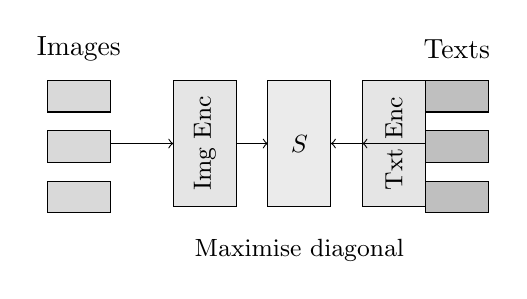
\begin{tikzpicture}[scale=0.8]
    % Images
    \node at (0,3) {Images};
    \foreach \i in {0,1,2} {
        \draw[fill=black!15] (-0.5,2-\i*0.8) rectangle (0.5,2.5-\i*0.8);
    }

    % Image encoder
    \draw[fill=black!10] (1.5,0.5) rectangle (2.5,2.5);
    \node[rotate=90] at (2,1.5) {\small Img Enc};

    % Text
    \node at (6,3) {Texts};
    \foreach \i in {0,1,2} {
        \draw[fill=black!25] (5.5,2-\i*0.8) rectangle (6.5,2.5-\i*0.8);
    }

    % Text encoder
    \draw[fill=black!10] (4.5,0.5) rectangle (5.5,2.5);
    \node[rotate=90] at (5,1.5) {\small Txt Enc};

    % Similarity matrix
    \draw[fill=black!8] (3,0.5) rectangle (4,2.5);
    \node at (3.5,1.5) {\small $S$};

    % Arrows
    \draw[->] (0.5,1.5) -- (1.5,1.5);
    \draw[->] (5.5,1.5) -- (4.5,1.5);
    \draw[->] (2.5,1.5) -- (3,1.5);
    \draw[->] (4.5,1.5) -- (4,1.5);

    % Diagonal
    \node at (3.5,-0.2) {\small Maximise diagonal};
\end{tikzpicture}
\caption{CLIP training: maximise similarity between matching image-text pairs along the diagonal.}
\label{fig:clip_training}
\end{figure}

\subsection{Zero-Shot Classification with CLIP}

\begin{algorithm}[H]
\caption{CLIP Zero-Shot Classification}
\begin{algorithmic}[1]
\Require Image $x$, class names $\{c_1, \ldots, c_K\}$, prompt template $T$
\For{each class $k$}
    \State $t_k \gets T(c_k)$ \Comment{e.g.\ ``a photo of a \{class\}''}
    \State $e_k \gets f_{\text{text}}(t_k)$ \Comment{Text embedding}
\EndFor
\State $e_x \gets f_{\text{image}}(x)$ \Comment{Image embedding}
\State $\hat{y} \gets \arg\max_k \cos(e_x, e_k)$
\end{algorithmic}
\end{algorithm}


\section{Prompt Engineering}\index{prompt engineering}

\marginnote{The prompt is the new hyperparameter.}

\newthought{The choice of text prompt} significantly affects performance:

\begin{table}
\centering
\begin{tabular}{lc}
\toprule
\textbf{Prompt} & \textbf{Accuracy} \\
\midrule
``\{class\}'' & 58.2\% \\
``a photo of a \{class\}'' & 63.5\% \\
``a photo of a \{class\}, a type of pet'' & 67.1\% \\
Ensemble of 80 prompts & 76.2\% \\
\bottomrule
\end{tabular}
\caption{Prompt engineering effects on ImageNet zero-shot accuracy.}
\label{tab:prompt_engineering}
\end{table}

\newthought{Prompt ensembling} averages embeddings from multiple prompt templates.

\newthought{CoOp}\index{CoOp} learns soft prompt tokens via gradient descent~\cite{Zhou2022CoOp}:
\begin{equation}
    t = [V_1][V_2]\ldots[V_M][\text{class}]
\end{equation}
where $V_i$ are learnable embeddings.


\section{Few-Shot Learning}\index{few-shot learning}

\marginnote{Few-shot: learn from 1--5 examples per class.}

\subsection{Fine-tuning Approaches}

\newthought{Linear probing}\index{linear probe} freezes the encoder and trains a linear classifier. Full fine-tuning updates all parameters but risks overfitting. Adapters\index{adapter} add small trainable modules while freezing the rest of the network.

\subsection{In-Context Learning}\index{in-context learning}

\newthought{Large language models} can do few-shot via prompting: provide a few input-output examples in the prompt, then query for a new input. No gradient updates are needed; the model learns from the examples in context.


\section{Foundation Models}\index{foundation model}

\marginnote{Foundation models: large pre-trained models that serve as building blocks.}

\subsection{SAM: Segment Anything Model}\index{SAM}

\newthought{SAM} was trained on 1 billion masks from 11 million images~\cite{Kirillov2023SAM}. It is promptable via point, box, or text input, and achieves zero-shot segmentation of arbitrary objects.

\subsection{DINO: Self-Distillation with No Labels}\index{DINO}

\newthought{DINO} is a self-supervised vision transformer~\cite{Caron2021DINO} that learns semantic features without any labels. Its attention maps highlight object parts, making the learned representations highly interpretable.

\subsection{Composing Foundation Models}

\newthought{Combining} CLIP for understanding, SAM for segmentation, and Stable Diffusion for generation enables complex pipelines without task-specific training.


\section{Domain Adaptation}\index{domain adaptation}

\marginnote{What if training and test data come from different distributions?}

\subsection{Types of Shift}

\newthought{Covariate shift}\index{covariate shift} occurs when $P(X)$ changes but $P(Y|X)$ stays the same. Label shift\index{label shift} occurs when $P(Y)$ changes but $P(X|Y)$ stays the same. Concept drift\index{concept drift} occurs when $P(Y|X)$ changes over time.

\subsection{Domain-Invariant Features}

\newthought{The goal} is to learn features that are informative for the task but indistinguishable between domains:

\begin{equation}
    \min_f \mathcal{L}_{\text{task}}(f) + \lambda \mathcal{L}_{\text{domain}}(f)
\end{equation}

where $\mathcal{L}_{\text{domain}}$ penalises features that reveal domain identity.

\subsection{Adversarial Domain Adaptation}\index{adversarial domain adaptation}

\newthought{An adversarial approach} trains a domain discriminator; the encoder tries to fool it~\cite{Ganin2016DomainAdversarial}:

\begin{figure}
\centering
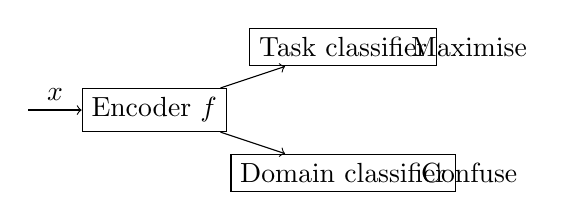
\begin{tikzpicture}[scale=0.8]
    \node[draw, rectangle] (enc) at (0,0) {Encoder $f$};
    \node[draw, rectangle] (task) at (3,1) {Task classifier};
    \node[draw, rectangle] (domain) at (3,-1) {Domain classifier};

    \draw[->] (-2,0) -- (enc) node[midway, above] {$x$};
    \draw[->] (enc) -- (task);
    \draw[->] (enc) -- (domain);

    \node at (5,1) {Maximise};
    \node at (5,-1) {Confuse};
\end{tikzpicture}
\caption{Adversarial domain adaptation: features should help the task but not reveal the domain.}
\label{fig:domain_adaptation}
\end{figure}


%───────────────────────────────────────────────────────────────────────
% SECTION 6: AI Engineering   (STUB --- TO DRAFT)
%───────────────────────────────────────────────────────────────────────
% Theme: concepts that matter when we reuse and DEPLOY large models we
% cannot really control through training. Sits at the bottom of Block 2
% as the operational counterpart to §1-§5.
%
% Tentative beats:
%   - Opener: the shift from training to operating (model arrives ready,
%     all the engineering effort moves to inference time and deployment).
%   - Retrieval-augmented generation (give the model facts at inference
%     instead of retraining; the encoder for retrieval is itself a backbone
%     callback to §1; the generator stays frozen).
%   - Tool use and agents (give the model actions at inference; function
%     calling, agentic loops, multi-step orchestration; the model decides,
%     deterministic code executes).
%   - Evaluation when you didn't train: LLM-as-judge, behavioural / red-team
%     tests, eval harnesses, A/B testing in production. Standard ML metrics
%     are insufficient when the model was trained for a different objective.
%   - Guardrails and safety: input sanitisation, output validation, refusal
%     behaviour, prompt-injection / jailbreak resistance, content moderation
%     stacks. Each is a wrapper around a model the team did not train.
%   - Cost / latency / quality trade-offs: model selection (small vs large,
%     local vs API), prompt caching, speculative decoding, distillation,
%     quantisation. The same accuracy can usually be bought at very
%     different price points.
%   - Monitoring and drift: callback to ch07. Distribution shift in
%     production needs operational signals, not training-time signals,
%     because there is no fresh ground truth.
%   - Versioning and lineage: model cards, dataset cards, eval cards,
%     prompt versioning. When the model is a black box, provenance is the
%     only thing you can audit.
%
% Closing move: AI engineering is what fills the gap left by the fact that
% the team deploying the model is almost never the team that trained it.
% The operational discipline replaces the training-time control we used
% to take for granted.
%───────────────────────────────────────────────────────────────────────

\newpage
\section{AI Engineering}\index{AI engineering}\index{retrieval-augmented generation}\index{guardrails}

\marginnote{\newthought{TODO: draft this section.} Stub only. Outline lives in the comment block above; budget ~150 lines in the final draft.}

\newthought{The chapter so far} has assumed that we control the model through training. AI engineering is what becomes important when we do not.

\vspace{2.5em}


%═══════════════════════════════════════════════════════════════════════
% BLOCK 3: STUDENT ACTIVATION
%═══════════════════════════════════════════════════════════════════════

\newpage
\section{Examples \& Exercises}

\subsection{Exercise 1: Zero-Shot with CLIP}

You want to classify images into \{beach, mountain, city, forest\}.

\begin{enumerate}
    \item Write 3 different prompt templates.
    \item How would you ensemble them?
    \item What if ``forest'' and ``mountain'' are often confused?
\end{enumerate}

\subsection{Exercise 2: Few-Shot Fine-tuning}

You have 5 examples per class for a 10-class problem, 50 examples total.

\begin{enumerate}
    \item Why might full fine-tuning fail?
    \item What regularisation would you use?
\end{enumerate}

\subsection{Exercise 3: Domain Shift}

Your model trained on ImageNet performs poorly on medical X-rays.

\begin{enumerate}
    \item What type of domain shift is this?
    \item Propose two solutions.
\end{enumerate}

\fi
\section{Self-Reflection and Recap}

\newthought{Self-Reflection.}

\begin{enumerate}
    \item Why does CLIP generalise to unseen categories?
    \item When does fine-tuning outperform zero-shot, and when is the reverse true?
    \item How does prompt ensembling reduce the sensitivity to a single prompt choice?
    \item What makes CoOp's learned prompts more effective than hand-crafted ones?
    \item When would you prefer a linear probe over full fine-tuning for few-shot tasks?
    \item How does adversarial domain adaptation differ from simply fine-tuning on target data?
    \item What risks arise when composing multiple foundation models in a pipeline?
\end{enumerate}

\vspace{1.5em}

\newthought{Recap.}

\begin{itemize}
    \item Transfer learning reuses pre-trained features; early layers transfer well, but late layers require adaptation, and large domain gaps risk negative transfer.
    \item Zero-shot classification via CLIP matches image embeddings to text prompt embeddings; prompt design and ensembling are critical for accuracy.
    \item Few-shot strategies range from linear probing to full fine-tuning; the right choice depends on how much labelled data is available and how far the target domain is from the source.
    \item Domain adaptation techniques learn features that are informative for the task but invariant to the domain, mitigating covariate shift.
    \item Foundation models such as CLIP, SAM, and DINO serve as composable building blocks for tasks they were never explicitly trained on.
\end{itemize}

\vspace{2.5em}

\marginnote{\newthought{Root cause.} Every method in this chapter assumes the backbone already exists. Pretraining is treated as someone else's problem; the next chapter shows whose problem it is and how it gets solved without labels.}

\newthought{The backbone arrives ready-made.} Throughout this chapter we have taken pretrained encoders as given and asked how to reuse them. ImageNet supervised pretraining works for natural images because someone else once labelled fourteen million examples, but no second ImageNet is being built for every new domain. Foundation models such as CLIP escape this bottleneck not by labelling more, but by extracting supervision from data that was already there, in the form of image-caption pairs scraped from the web. The supervision was hiding in plain sight.

\newthought{Self-supervised learning} generalises this idea. Instead of asking humans for labels, the model is given a task that can be solved using only the structure of the data itself: predict the masked patch from the surrounding patches, pull augmented views of the same image close together, predict the next token from the previous ones. The labels come from the data, and the representations that emerge are the very backbones this chapter has taught us to reuse.

\marginnote{\newthought{Teaser.} If we already have the data, where in the data do the labels hide?}

\newthought{The next chapter explores} how data structure becomes its own supervision signal, walking through the contrastive and predictive families of self-supervised objectives that produced the foundation models we have just learned to reuse.

\marginnote{\newthought{feedback}}
